\section*{Question 2}

\renewcommand{\thefigure}{11}
\begin{figure}[h!]
    \centering
    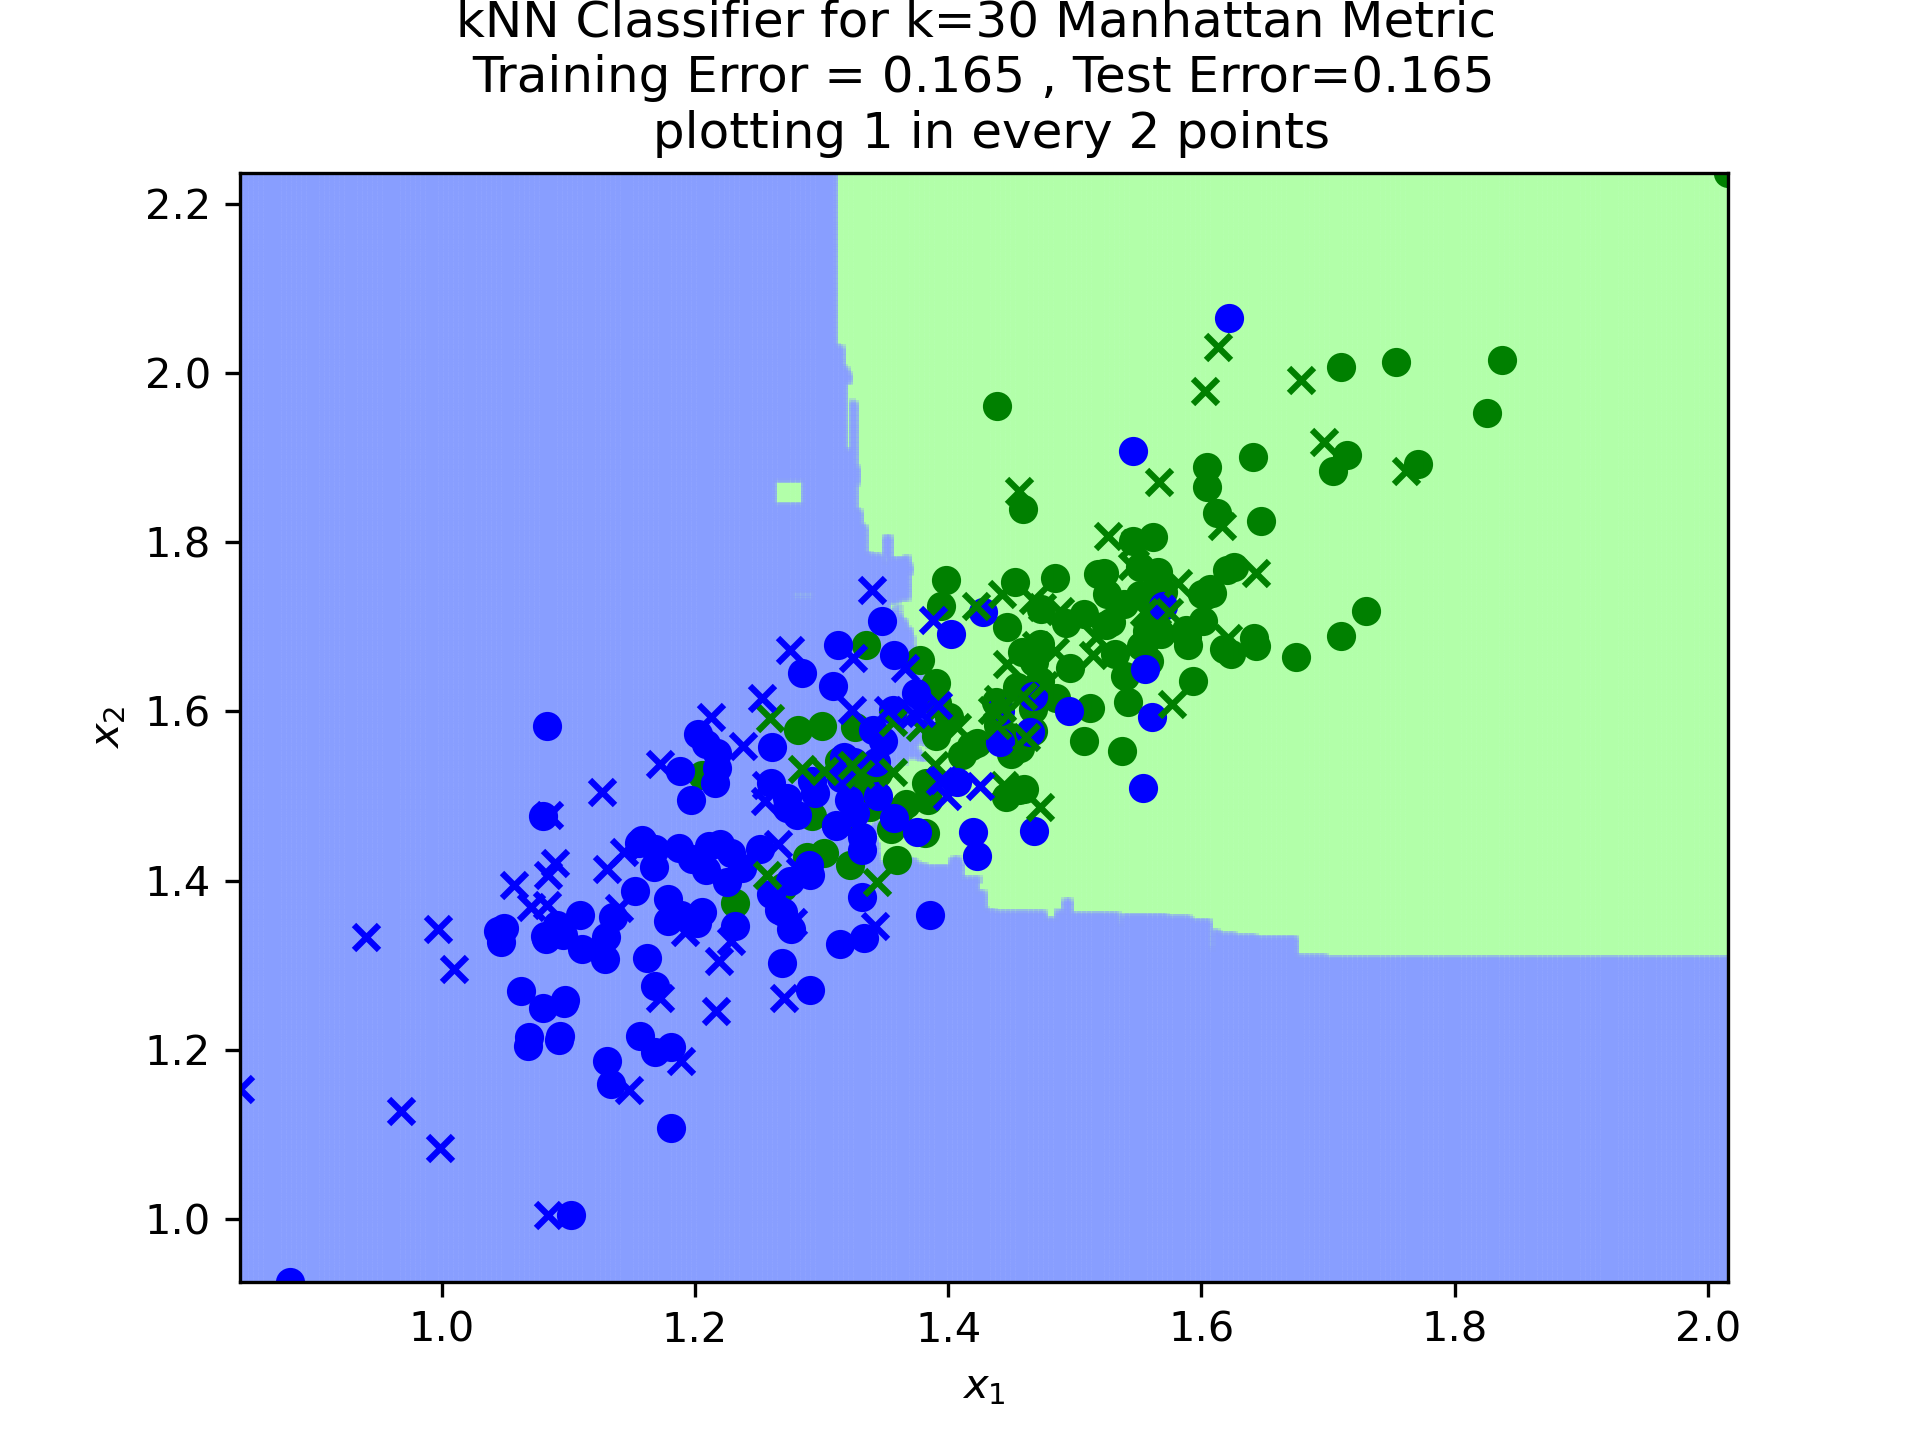
\includegraphics[width=\singleWidth]{Graphs/Q2_single.png}
    \caption{kNN classifier for k=30 using the {\bf Manhattan} metric,
    sNC region in green, sDAT region in blue}
    \label{fig:Q2_single}
\end{figure}


As shown in the table \ref{tab:Q1errors}, k=30 was the best performing kNN classifier
for the {\it Euclidean} metric. We now compare this classifier with the equivalent
classifier using the {\it Manhattan} metric. 

Since the each feature vector has two features, the \textit{Euclidean} distance between two
features ($\bar{x}=(x_1, x_2)$ and $\bar{y}=(y_1, y_2)$) is given by equation
\ref{eq:euclid}, and the \textit{Manhattan} distance is given by equation \ref{eq:man}.
The boundary visualization graph for the Manhhattan metric is provided in figure \ref{fig:Q2_single}.
The ``blocky'' nature of the Manhattan metric is visible in the boundary division between the two
evaluated classes (sNC and sDAT).


\begin{equation}
  D_{\text{Euclidean}} = \sqrt{(x_1 - y_1)^2 + (x_2 - y_2)^2}
  \label{eq:euclid}
\end{equation}

\begin{equation}
  D_{\text{Manhattan}} = |x_1 - y_1| + |x_2 - y_2|
  \label{eq:man}
\end{equation}


The {\it Euclidean} metric resulted in a training error of $err_{\text{Euclidean}}=0.169$, and
a tersting error over the given test data set is $Err(D)_{\text{Euclidean}}=0.160$.
For the {\it Manhattan} metric, the training error
is $err{\text{Manhattan}}=0.165$,
and the testing error is over the same data set is $Err(D)_{\text{Manhattan}}=0.165$.
The {\bf Euclidean} metric has a {\bf better performance}
than the Manhattan metric in this given test data set. This suggests that the kNN classifier
generalizes better with the Manhattan metric, specially considering that the {\bf training error}
is lower for the Manhattan metric, even though it's generalized error is worse.
